\section{Evaluation}

This section presents an in-depth empirical analysis of the design discussed in
Section~\ref{design-section}. To this end, we assess the scalability and
efficiency of the solution using multiple criteria.
%
First, an evaluation of the strong scaling behavior of the distributed
algorithm is presented.
%
Second, the weak scaling of the solution is assessed with respect to increasing
numbers of targeted latent communities.
%
Next, the effects of varying the number of latent communities on the system's
performance is analyzed.
%
Further, we evaluate the efficiency and overhead associated with network
communication between cluster nodes.
%
Finally, we contrast the effectiveness of scaling the computation horizontally
and vertically.

Empirical results were obtained by performing experiments on the VU and TU/D
DAS5 clusters which consist of 68 and 48 compute nodes respectively. Each
compute node is equipped with a dual 8-core Intel Xeon E5-2630v3 CPU clocked
at 2.40GHz, 64GB of memory and 8TB of storage. Moreover, the compute nodes of
each site are interconnected by an internal 1~Gbit/s Ethernet and FDR~InfiniBand.

\subsection{Strong scaling}

\begin{figure}[ht] % [htb]
  \centering
  \epsfig{file=plots/sweep-over-np-fixed-K.eps, width=\columnwidth}
  \caption{Strong scaling: varying the number of compute nodes for a fixed
  problem size.}
  \label{fig-strong-scaling}
\end{figure}

\subsection{Weak Scaling}

\begin{figure}[t] % [htb]
  \centering
  \epsfig{file=plots/sweep-over-K-proportional-np.eps, width=\columnwidth}
  \caption{Weak scaling: varying the number of compute nodes proportionally to
  the number of latent communities.}
  \label{fig-weak-scaling}
\end{figure}

\subsection{Effects of Number of Communities on Performance}
\begin{figure}[t] % [htb]
  \centering
  \epsfig{file=plots/sweep-over-K-fixed-np.eps, width=\columnwidth}
  \caption{Effects of varying the number of communities on the algorithm's
  throughput.}
  \label{fig-throughput}
\end{figure}

\subsection{Horizontal vs. Vertical Scalability}
\begin{figure}[t] % [htb]
  \centering
  \epsfig{file=plots/hpc-cloud.eps, width=\columnwidth}
  \caption{FIXME}
  \label{fig-ppx-cpu}
\end{figure}

\subsection{Cluster Communication Efficiency}

\subsection{Convergence of Large Datasets}
\begin{figure*}[t] % [htb]
  \centering
  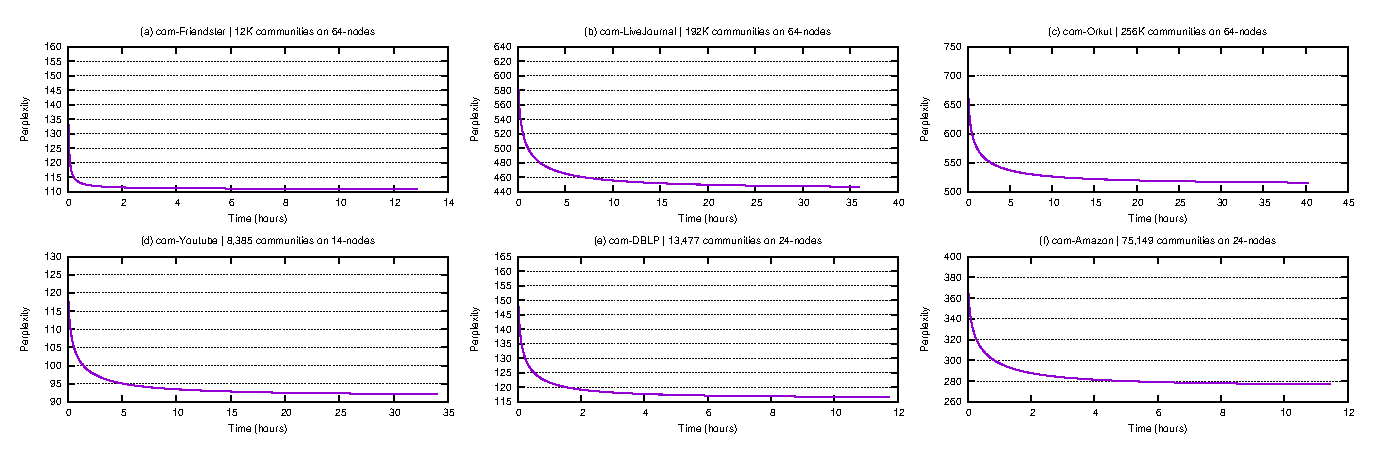
\epsfig{file=plots/ppx.eps, width=\textwidth}
  \caption{FIXME}
  \label{fig-ppx-cpu}
\end{figure*}

